\updatehighlight{
    name=accentB,
    add={\section}
}

\addtorecentlist{\textbackslash subsection}
\begin{saveblock}{sectionCommands}
    \begin{highlightblock}[linewidth=0.5\textwidth,gobble=8]
        \section{AA}
        Lorem ipsum dolor sit amet,
        consectetur adipiscing elit.
        
        \section{BB}
        \subsection{CC}
        \subsubsection{DD}
        \subsection{EE}
        Nullam a risus at arcu
        lobortis viverra vel
        volutpat diam.
        
        \section{FF}
        \subsubsection{GG}
        ~~
    \end{highlightblock}
\end{saveblock}

\begin{frame}[fragile]
    \frametitle{Section commands}

    \begin{columns}
        \begin{column}{0.5\textwidth}
            % \useblock{sectionCommands}
            \begin{codebox}
                \begin{minted}{tex}
                    \section{AA}
                    Lorem ipsum dolor sit amet,
                    consectetur adipiscing elit.
                    
                    \section{BB}
                    \subsection{CC}
                    \subsubsection{DD}
                    \subsection{EE}
                    Nullam a risus at arcu
                    lobortis viverra vel
                    volutpat diam.
                    
                    \section{FF}
                    \subsubsection{GG}
                \end{minted}
            \end{codebox}
        \end{column}
        \begin{column}{0.5\textwidth}
            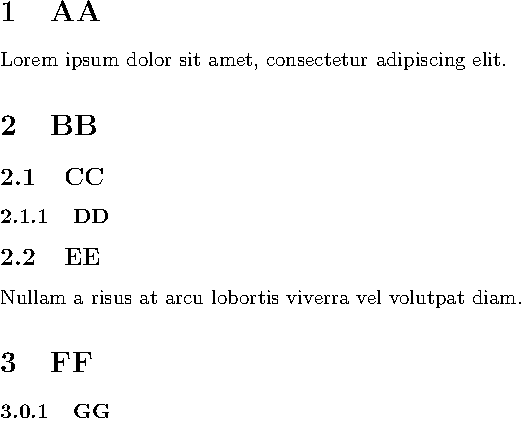
\includegraphics[width=\linewidth,height=0.8\textheight,keepaspectratio]{assets/sectioncommands.pdf}
        \end{column}
    \end{columns}
\end{frame}

\updatehighlight{
    name=accentB,
    remove={\section}
    %
    name=default,
    add={\section}
}
